\documentclass[jou,apacite]{apa6}

\title{Applying Recursion and Fractals As Design Patterns In Complex Systems}
\shorttitle{Term Paper}

\author{Steve Mazza}
\affiliation{Naval Postgraduate School}

\abstract{
  We introduce complexity and show some common methods for dealing with it, namely abstraction and encapsulation.  We then show how applying recursive thinking to complex systems reduces the complexity of their description, illustrated with an example from computer science.  We make a connection from recursion to fractals, introducing some common types and showing how they relate to real world concepts.  Introducing the use of design patterns in architecture, we discuss some of its history and applicability to systems engineering.  We show how shortcomings in traditional design patterns fail to adequately deal with complex systems in a highly effective manner.  We make the link to recursive descriptions of patterns which can be found in some classes of fractals.  Fractal-based patterns that are specifically designed to address the unique needs of the systems engineer regarding the architecture of complex systems will shorten the gap between problem observation and problem solution while also increasing the reliability and repeatability of success in these domains.
}

\rightheader{Term Paper}
\leftheader{Steve Mazza}

\begin{document}
\maketitle    
                        
\section{Introduction}  % Target: 1 page
We introduce complexity and show some common methods for dealing with it, namely abstraction and encapsulation.  We then show how applying recursive thinking to complex systems reduces the complexity of their description, illustrated with an example from computer science.  We make a connection from recursion to fractals, introducing some common types and showing how they relate to real world concepts.

Introducing the use of design patterns in architecture, we discuss some of its history and applicability to systems engineering.  We show how shortcomings in traditional design patterns fail to adequately deal with complex systems in a highly effective manner.  We make the link to recursive descriptions of patterns which can be found in some classes of fractals.  There exists an analog between certain fractals and the recursive descriptions for complex problems that we can leverage in
the interest of taming complexity on some levels.

The natural extension is the full development of useful and descriptive recursive fractal-based patterns that are specifically designed to address the unique needs of the systems engineer regarding the architecture of complex systems.  While this will take time and research, the benefits of this endeavor promise to shorten the gap between problem observation and problem solution while also increasing the reliability and repeatability of success in these domains.

\section{Background}  % Target: 2 pages
The paper that follows is predicated on developing a working understanding of complexity in the context in which we intend.  Furthermore, we arrive at a common understanding of how to describe complex systems.  And lastly, we introduce the idea of recursion and show how it is able to simplify our description of systems (or problems) in many instances.

\subsection{What Is Complexity?}  % Target: 1/2 page.
What is complexity?  What is the character that makes some systems complex and others not?  Is there a hard line between complexity and non-complexity or do we just know it when we see it?\footnote{This is a clear reference to Justice Stewart's description of pornography.  The point is, can complexity be definitely identified (as in the legal sense) or is its character more elusive?}

At the root, problems are complex when they are difficult to understand or predict.  Murray Gell-Mann proposed that systems should be considered complex when the difficulty in predicting their outcome is due, not to irregularities (or randomness), but to regularities in the system that are difficult to describe.  This, he suggests, differentiates between purely random outcomes which are not necessarily complex and complex systems whose outcomes are difficult to
predict.~\cite{GellMann}

Miller counters that there should possibly not be any single unified definition of complexity, arguing that trying to unify them may be asking too much.
\begin{quotation}
  Complexity can occur at many levels, including time, space, and interactions.  Perhaps we are expecting too much if we want a single measure of complexity that captures all of our intuitions.~\cite[page 234]{Miller}
\end{quotation}

Miller is, of course not wrong.  But despite the fact that there are several ways in which we can think about complexity, we will still benefit from a working definition.  So we will adopt the definition proposed by Mitchell in which, ``large networks of components with no central control and simple rules of operation give rise to complex collective behavior, sophisticated information processing, and adaptation via learning or evolution.''~\cite[page 13]{Mitchell}

Many researchers will agree that it is the interactions among the moving parts of a system that are instrumental in giving rise to complexity.  Langford characterizes interaction as, ``the transfer of something from one object (sender) to another object (receiver).''~\cite[page 48]{Langford}  This is a transfer of information which can be used to influence behavior or decisions or to affect internal change (i.e., state change).  Axelrod and Cohen argue that it is interactions that, ``make a Complex Adaptive System come alive.''~\cite[page 63]{Axelrod} They devote an entire chapter to their importance, arguing that interactions afford opportunities for information exchange, without which system complexity is significantly reduced.  

The concept of complexity might be best illustrated with a counter-example.  At first glance, one might consider a mechanical wrist watch to be a highly complex instrument.  In fact, it is not complex at all; merely complicated.  The interactions among its parts is so highly constrained (pre-ordained) that complexity cannot arise.  Robustness, a hallmark of complexity, is missing entirely.  If one were to remove a piece of the instrumentation (e.g., a gear or spring) the wrist watch
would cease to operate.

\subsection{How to Describe Complex Systems}  % Target: 1/2 page.
Formal methods are the basis by which we achieve repeatability in engineering.  Without them we are doomed to fumble around in the dark, revisiting the same mistakes on successive efforts.  Frameworks such as the Department of Defense Architecture Framework (DoDAF) and The Open Group Architecture Framework (TOGAF).  

These provide the basis for structured, disciplined engineering and help guide and support the full life cycle of development.  They help us to manage and understand our engineering design problems within the context of the broader support for their development, use, and disposal but they do not contain tools that are specific to decomposing the understanding of and communicating the complexity at the root of our design challenges.

The design patterns that we use are tools that help us visualize, understand, and communicate complexity in a relatively standardized manner.  They describe recurring problems along with the core of their solution.  Inasmuch they provide an easy way of rapidly transferring large amounts of information about a problem in an accessible way.  In order to keep pattens useful in a standardized way, the Gang of Four\footnote{This is a commonly used reference to Gamma, Helm, Johnson, and Vissides and to their 1994 treatise on design patterns.} describe four essential elements of any design pattern: the pattern name, the problem, the solution, and the consequences.~\cite[page 3]{Gamma}

\subsubsection{Pattern Name}
Providing a name for our pattern facilitates rapid communication of complex ideas by increasing our design vocabulary.  Agreeing on a name means that engineers across many different problem domains can refer to the same problem and solution without ambiguity.

\subsubsection{Problem}
Very simply, the problem describes when and how we can apply the pattern.  It provides the context for the pattern's use and may also set some conditions which must be met in order to do so.  The problems to which patterns apply may occur at any level of design.  The problem may be specific or may be descriptive of a whole class of design ideas.

\subsubsection{Solution}
The solution is sufficiently abstract such that it can be applied to a a range of implementations.  The solution should describe the elements of the design and their interactions.\footnote{Recall the importance of interactions in complex systems.}  It may also describe the relationships and responsibilities of elements within the design.

\subsubsection{Consequences}
These are the critical basis for evaluating design decisions and involve trade offs such as flexibility, adaptability, speed, cost, and time.  They are critical for choosing the correct alternatives when using patterns.  Because consequences are not always  listed explicitly within the description of a pattern, a thorough understanding of that pattern is necessary in order to evaluate its use.

The use of design patterns in software engineering is fairly ubiquitous.  Design patterns in other disciplines varies, but is potentially equally as applicable.  The emerging field of systems engineering has many analogs in software engineering and, consequently, may benefit equally from the establishment of a set of commonly accepted design patterns as the basis for a design vocabulary.

Design patterns provide a way of simplifying difficult problems by packaging the problem, solution, and consequences into a neat package and providing a name (a handle) by which to refer to it.  This is a mechanism of abstraction and provides us with a very powerful tool for helping us deal with difficult and complex designs.

\subsection{Methods Of Simplifying Complexity}  % Target: 1/2 page.
There are two tools in our arsenal that gain us a lot of ground toward simplifying complexity.  They are abstraction and encapsulation and we introduce and discuss them here, first individually, and then show how we can put them together to provide a powerful way of thinking about difficult and complex problems.  The distinction between abstraction and encapsulation requires some working out since they are almost always used in conjunction.

\subsubsection{Abstraction}
Abstraction is the mechanism by which an interface to a potentially complex entity is simplified.  The term \emph{abstract} used as an adjective means existing in thought or as an idea but not having a physical or concrete existence.  This separation between the idea (or essence) of something and its implementation gets at the core of why we care about abstraction at all.  

It is very nice when trying to simplify a difficult problem to just concern ourselves with the interface, or contract, (see below) or even an idealized interface (at first) in order to gain an appropriate conceptual foothold on the complexity.  Since abstraction refers to showing only the necessary details of an interface to the consumer, it also provides us a mechanism by which we can ratchet up the complexity as our understanding of the problem space increases.

As an example, consider the act of shipping a parcel to a relative in another state.  Your responsibility as the consumer begins and ends with providing a valid shipping and return address and making payment.  You need not concern yourself with the underlying implementation of \emph{by what means} the package will arrive to your relative.  It could be conveyed via ground freight or travel by air or even be strapped to a donkey.  Assuming it arrives on time and in tact, you are afforded the luxury of not caring about the details\dots the implementation of its delivery.  If the shipper invented a teleportation machine, you would be none the wiser.\footnote{Although one would assume that the rates would go up in order to cover the research and development}.  The idea of \emph{shipping a parcel} is an abstraction on the mechanism of actually getting it to its destination.

\subsubsection{Encapsulation}
In contrast, encapsulation hides  data as well as complexity.  However the emphasis is not on the interface, but on providing \emph{data protection.}  Encapsulation literally means \emph{to surround.}  While the complexity of an entity is a function of its implementation, it is not the implementation details that are important to encapsulation, rather the data and complexity.  Protection in this case often refers to the prevention of access of data by users in unintended ways.  The mechanism of encapsulation enforces integrity of the type, entity, or object.

Proper encapsulation enforces the contract with the user regarding how an entity or artifact will respond to interaction with its interface.  Abstraction is the simplification of the interface; encapsulation is the hiding and protection of the data behind the interface.  It controls the means by which the artifact may be used.  Unlike abstraction, encapsulation often refers to a specific concrete implementation.

Consider the example of my morning coffee.\footnote{The author presents this statement as if there is only one morning coffee.  Subscription to this tenant is pure folly.}  Since the installation of the Kureg machine in our break room, the production of coffee requires me only to select the type of coffee I want, insert the capsule into the machine, and press the large \emph{Brew} button on the front.  I need not care about how much water is required,\footnote{The Kureg machine in our break room has a water line from the sink water supply so there is no reservoir to fill.} the temperature of that water, how to grind the coffee, or how long to steep the grounds.  Fortunately for me, the button on the face of the machine is an encapsulation of how to brew coffee.

\subsubsection{Putting Them Together}
Abstraction and encapsulation are natural partners in simplifying our understanding of complexity.  Taken together, they afford us a simultaneous simplification of the interface (i.e., contract with the user) and a protection of the implementation details.  This allows us to focus on the \emph{what} and temporarily ignore the \emph{how} of an entity or artifact.

In a more practical manner, the use of abstraction and encapsulation together allows the distributed design and development of a solution to a complex problem in a way that accommodates the natural development life cycles of individual component parts to progress at their own pace and schedule.  So long as the interface contract (abstraction) is maintained, the implementation details (encapsulation) are free to evolve as appropriate.

This leads us to a concept that is often referred to as \emph{black box} architecture.  It is a powerful mechanism for dealing with complexity and complex systems.  Design patterns are used by engineers to create an understanding of difficult systems (or problems) and to create a conceptual framework around that problem space that is descriptive of a solution.  The design patterns usually suggest natural divisions where interfaces can be created but remain agnostic of the details of implementation, leading to the black box architecture.  Thus abstraction and encapsulation naturally flow from the effective use of design patterns, making them well suited to reducing complexity.

\subsection{Introducing Recursion}  % Target: 1/2 page.
The joke goes that in order to understand recursion\footnote{See Recursion}, you must understand recursion.

\subsubsection{Definition of Recursion} % http://mathworld.wolfram.com/Recursion.html
    \begin{quote}
      ``A recursive process is one in which objects are defined in terms of other objects of the same type.''~\cite{Wolfram} 
    \end{quote}
    Very often the object of the same type is actually an exact copy of the first instance of the object but with a slightly different value, as in the case of a recursive algorithm in computer science.  Another instance of a given function gets pushed on the call stack but is passed a different parameter.

    The essence of recursion is that you may solve a large or difficult problem by first solving smaller versions of that same problem and applying those results to the larger problem.  Developing a recursive solution to a problem hinges on identifying a base case so that you know where to start or end. 

\subsubsection{Recursion in the Classroom}   % http://www.go4expert.com/articles/calculating-factorial-recursively-t1757/
This may be easiest to understand if we walk through an example.  We will first select an algorithmic example so that we can keep our discussion tidy.

A classic example of recursion can be shown in the implementation of the factorial algorithm, which calculates $n!$ where $n$ is some positive integer.  The factorial of $n$ is the product of $n$ and all the positive integers below it such that  

\[n!\equiv n(n-1)\cdots 2\cdot 1\]

For example, $3! = 3\times2\times1 = 6$.

Implementing this algorithm in the C programming language, we have
\begin{verbatim}
unsigned int iter_factorial(int n) {
  int f = 1;
  int i;
  for(i = 1; i <= n; i++) {
    f *= i;
  }
  return f;
}
\end{verbatim}
The implementation of this algorithm takes the integer argument $n$ and uses the loop variable $i$ to count from 1 to $n$, multiplying and collecting the loop variable in $f$.

Notice how much more streamlined the implementation and subsequent description are under a recursive version of the algorithm.
\begin{verbatim}
unsigned int recursive_factorial(int n) {
  return n>=1 ? n * recr_factorial(n-1) : 1;
}
\end{verbatim}
In this version, we are either multiplying $n$ by the previous result of the function call or returning the value 1.  The ternary operator looks menacing if you have not seen it, but what is happening (from left to right) is that $n$ is compared against 1 and while it is still greater than or equal to 1, another copy of the function is pushed onto the call stack with the new value $n-1$.  In this way the values passed to the successive copies of the function march inexorably toward
the terminal state, 1, at which point the final value is eventually returned.

Notice in this construction, we are calling the function from within the function, itself.\footnote{Within a typical computing environment this is possible because each successive call to the function pushes the previous calls one level deeper on the stack and so variable name space is preserved.}

\subsubsection{Recursion in the Real World}  % http://sob.apotheon.org/?p=1814
While we will discuss the applicability of different proposed patterns later, we present here a common example in the interest of exposition.  Consider the task of processing a bill-of-materials, as in the case of manufacturing. The cost of a manufactured assembly (component) is the sum of the cost of component parts plus any associated labor and other overhead. However, the component parts themselves may be manufactured assemblies.  For example, an electric drill, made up
of a motor, chuck, bearings, housing, switch, and a cord. A motor is made up of a frame, stator, rotor, and bearings.  A rotor is made up of a shaft, stampings, wire, etcetera.

There are many examples of business processes that can be naturally expressed recursively.  Organizational charts, directories, and call trees are some.  The underlying implementations on which enterprise relational database management systems (RDBMS) are constructed are self-similar.  While B-Trees and B+Trees\footnote{These are simpler constructs which are often introduced in undergraduate computer science curricula.} are overly simple for robust commercial RDBMS, they are
exemplary of recursive constructs in the real world.

\section{Fractals}  % Target: 3 pages
In his 1983 treatise on fractal geometry, Benoit Mandelbrot introduced the scientific community to the greatest exposition on fractals to date, bringing fractal geometry into the collective scientific conscience.
\begin{quote}
  ``I conceived and developed a new geometry of nature and implemented its use in a number of diverse fields.  It describes many of the irregular and fragmented patterns around us, and leads to full-fledged theories, by identifying a family of shapes I call \emph{fractals}.''~\cite{Mandelbrot}
\end{quote}

Notice his use of language.  Mandelbrot talks about how fractals describe many of the things (ideas, systems, patterns) around us.  

\subsection{Self-similarity and Fractals}
Fractals are self-similar in nature.  It is an underlying theme with fractals.  That is, their construction looks the same (or similar) at varying levels of magnification.  As an illustration of this point, let us consider something with which we are all likely familiar.  Cauliflower offers an easy and accessible means to demonstrate self-similarity.  

\begin{figure}[htpb]
  \centering
  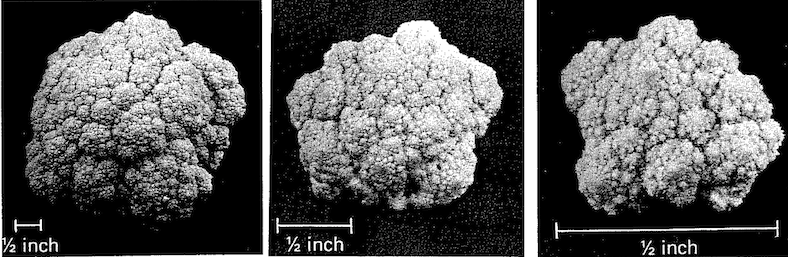
\includegraphics[width=\columnwidth]{images/cauliflower.png}
  \caption{The self-similarity of cauliflower demonstrated at three magnifications.}
  \label{fig:cauliflower}
\end{figure}

What is striking in figure~\ref{fig:cauliflower} is how remarkably alike each of the images is to the others.  Only the scale indicated on each frame gives away how large or small each piece of cauliflower is.

It is the same with fractals.  Each successive level of magnification reveals the same (or remarkably similar, in some cases) image as previously seen.  What we see in figure~\ref{fig:fractalmag} is a Sierpinski Gasket.  One third of it has been enlarged to show that it is indistinguishable from the whole, of which it is only a part.  

\begin{figure}[htpb]
  \centering
  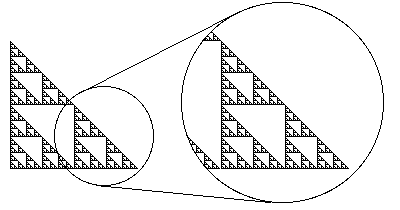
\includegraphics[width=\columnwidth]{images/GasketMag.png}
  \caption{Sierpinski Gasket illustrating self-similarity at different levels of magnification.}
  \label{fig:fractalmag}
\end{figure}

In fact, we have no real way of knowing (short of some external context) of we are looking at a whole or a small part or even a very, very tiny part of many fractals.  The self-similarity of fractals naturally lends itself to recursive description.

\subsection{Constructing Fractals}
Let us illustrate the self-similarity of fractals by constructing one in detail.  We will be developing the high level construction of others below, but it is useful to walk through a representative example.

For most fractal constructions what we require is a base case and an iterator, or rule, which we continually apply.  The iterator transforms the base case into something which often bares little resemblance to the original thing.

We will be looking at the Koch Curve whose base case is a single line segment, usually drawn horizontally as in figure~\ref{fig:koch0}.
\begin{figure}[htpb]
  \centering
  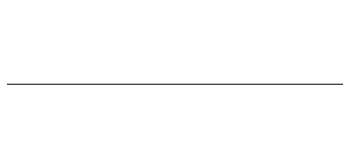
\includegraphics[width=0.75\columnwidth]{images/Koch0.png}
  \caption{Base case for the Koch Curve.}
  \label{fig:koch0}
\end{figure}

The iterator rule says to remove the center third of the line segment and replace it with an equilateral triangle.  Then take away its base.  This can be seen in figure~\ref{fig:kochiter}.
\begin{figure}[htpb]
  \centering
  
\includegraphics[scale=1.0]{images/KochIterationRule.png}
  \caption{Iteration rule for the Koch Curve.}
  \label{fig:kochiter}
\end{figure}
This obviously results in the curve shown in figure~\ref{fig:koch1}.
\begin{figure}[htpb]
  \centering
  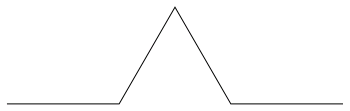
\includegraphics[width=0.75\columnwidth]{images/Koch1.png}
  \caption{Koch Curve after one iteration.}
  \label{fig:koch1}
\end{figure}
After the first iteration we continue to apply the rule individually to the four line segments, removing their center third, adding the equilateral triangle, and removing the base as shown in figure~\ref{fig:koch2}.
\begin{figure}[htpb]
  \centering
  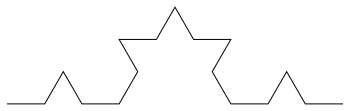
\includegraphics[width=0.75\columnwidth]{images/Koch2.png}
  \caption{Koch Curve after two iterations.}
  \label{fig:koch2}
\end{figure}
Successive iterations continue to result in a bumpier curve as illustrated in figure~\ref{fig:koch5}.
\begin{figure}[htpb]
  \centering
  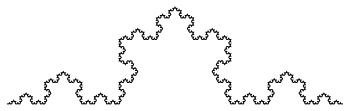
\includegraphics[width=0.75\columnwidth]{images/Koch5.png}
  \caption{Koch Curve after five iterations.}
  \label{fig:koch5}
\end{figure}

Notice that we are only continuing to apply the iterator to each successively smaller line segment in the curve.  It is the same rule applied over and over.  We can see how the simple iterator rule transforms a simple line segment into a very interesting curve with self-similar properties at all levels of magnification.

Of further interesting note is the observation that if the Koch Curve is drawn as three connected curves into a closed form, it creates a shape called a Koch Snowflake in which a boundary of infinite length\footnote{The iterator rule can always be applied between any two points of arbitrarily close proximity, creating new intermediate points.} surrounding a finite area\footnote{Since it is a closed curve, the area must be finite.}.

Since this is merely interesting and not crucial to our progress, we will leave the derivation of the following results to the reader.  The perimeter, $P$, a function of the length of a side, $s$, grows to infinity as the number of iterations, $n$, approaches infinity.

\[\lim_{n \to +\infty}P_n = \lim_{n \to +\infty} 3\cdot s\cdot\left(\frac{4}{3}\right)^n\to\infty\]

And the area, $A$, is finitely bound as the number of iterations, $n$, approaches infinity.

\[\lim_{n \to +\infty}A_n = \lim_{n \to +\infty}\frac{a_0}{5}\cdot\left(8-3\left(\frac{4}{9}\right)^n\right)=\frac{8}{5}\cdot a_0\]
where $a_0$ is the original area of the equilateral triangle.

\subsection{Selected Fractals}
We briefly introduce several of the more useful fractals, describe their construction, and provide illustrations.  We also provide a brief glimpse into the natural world constructs to which they may be applicable.~\cite{Peitgen} Consider each of the following examples and notice the role that recursive iteration plays.

\subsubsection{The Cantor Set}
The Cantor Set belongs to a class known as line elimination fractals.  We begin with a single horizontal line and continually remove the middle third (as in the Koch Curve), except that we do not add anything in its place.  Continuing to iterate this idea, the original line disappears into dust as more and more of it are continually removed.  The result is an uncountable set of measure zero.  Its construction is shown in figure~\ref{fig:cantor}.

\begin{figure}[htpb]
  \centering
  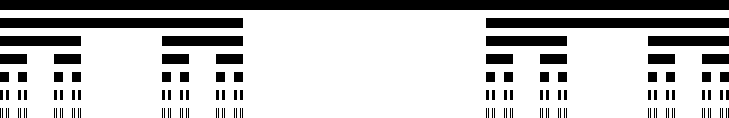
\includegraphics[width=0.75\columnwidth]{images/cantorset.png}
  \caption{Cantor Set showing six iterations.}
  \label{fig:cantor}
\end{figure}

The Cantor Set constructed on the interval $[0, 1]$ has the same cardinality as the real numbers on that same interval.  Inasmuch, we will find this pattern to be useful in representing closed, uncountable sets.  While the physical manifestation of these are few, the idea is quite a common theme, conceptually, in engineered systems of nontrivial complexity.

\subsubsection{The Sierpinski Gasket}
The Sierpinski Gasket belongs to a class known as area elimination fractals.  An equilateral triangle is divided into quarters by bisecting the midpoints of its line segments (sides) and the middle triangle is removed, leaving three equilateral triangles in its place.  The process is repeated \emph{ad infinitum} leaving something that looks like a gasket.  See figure~\ref{fig:sierpinski}.

\begin{figure}[htpb]
  \centering
  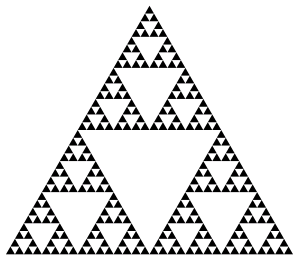
\includegraphics[width=0.75\columnwidth]{images/sierpinski.png}
  \caption{Sierpinski Gasket after five iterations.}
  \label{fig:sierpinski}
\end{figure}

Like the Cantor Set, there will always remain definite and identifiable points (endpoints, or boundaries) along the edges of the triangles.  As a pattern, there are potential applications in population growth and resource usage in biological systems, among others.

\subsubsection{The Pascal Triangle}
The Pascal Triangle is somewhat different in nature than the previous (or successive) examples in that its construction is purely computational and not as visually compelling, geometrically. An example is shown in figure~\ref{fig:pascal}. You can verify that it has the following three properties:
\begin{itemize}
  \item The sum of the $n^{\mbox{th}}$ row is $2^n$.
  \item The sum of rows 0 through $n$ is $-1+2^{n+1}$.
  \item The generating function of the $n^{\mbox{th}}$ row is $(x+1)^n$.
\end{itemize}

\begin{figure}[htpb]
  \centering
  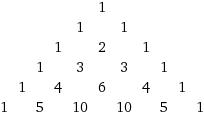
\includegraphics[width=0.75\columnwidth]{images/pascal.png}
  \caption{Pascal Triangle at $n=6$.}
  \label{fig:pascal}
\end{figure}

In 1654 Pascal, along with Pierre do Fermat, used his triangle to help solve some problems of chance as they related to gambling.  There are likely many similar applications of this pattern to stochastic outcomes in complex systems.

\subsubsection{Koch Curve}
Since we've already discussed this at some length above, we will simply mention that the Koch Curve belongs to a class called line replacement fractals.  This is one of the more recognizable and fascinating fractal structures and, in its closed form, bares a remarkable resemblance to a range of organic and natural structures, most notably snowflakes.

\begin{figure}[htpb]
  \centering
  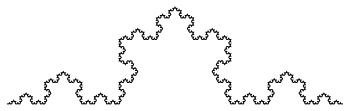
\includegraphics[width=0.75\columnwidth]{images/Koch5.png}
  \caption{Koch Curve after five iterations.}
  \label{fig:koch52}
\end{figure}

Because of its construction and infinitely increasing perimeter, it is an excellent analog (or pattern) for representing how accuracy in measurement, especially of organic or naturally occurring boundaries, impacts the results of that measurement.  Accuracy and an increase in length go proportionally, for example.  The classic illustration of this can be found in the 1967 article published in the journal \emph{Science}, titled, ``How Long is the Coast of
Britain?''\cite{Britain}

\begin{figure}[htpb]
  \centering
  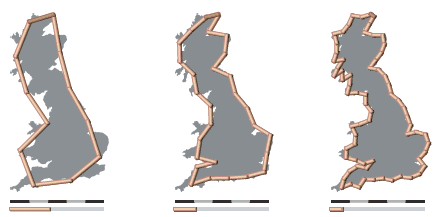
\includegraphics[width=0.75\columnwidth]{images/britain.png}
  \caption{From ``How Long is the Coast of Britain?'' this graphic is illustrative of how precision in measurement can affect its outcome.}
  \label{fig:britain}
\end{figure}

As illustrated in figure~\ref{fig:britain}, notice how the outcome of measurement of highly irregular shapes can be significantly affected by the accuracy, or precision, applied to that measurement.  At the risk of hyperbole, consider how the coastline would expand if one were able to account for irregularities as small as a grain of sand.

\subsubsection{Space Filling Curves}
The example shown in figure~\ref{fig:hilbert} is a Hilbert Curve, a member of the space filling curves.  Its construction can be seen in figure~\ref{fig:hilbert2}.  

\begin{figure}[htpb]
  \centering
  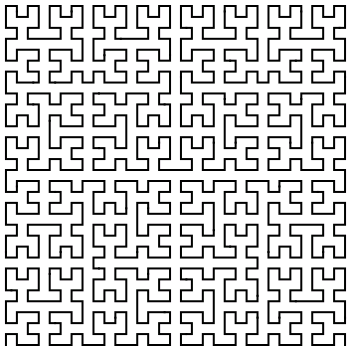
\includegraphics[width=0.75\columnwidth]{images/hilbert.png}
  \caption{Hilbert Curve after five iterations.}
  \label{fig:hilbert}
\end{figure}

One can see that the density increases rapidly with successive iterations.  For any arbitrary point in the plane, we can show that it will eventually be covered by the curve.

\begin{figure}[htpb]
  \centering
  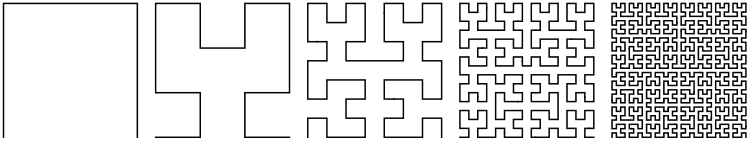
\includegraphics[width=0.75\columnwidth]{images/hilbert2.png}
  \caption{Construction of the Hilbert Curve.}
  \label{fig:hilbert2}
\end{figure}

Other examples of space filling curves include the Paeno Curve, Dragon Curve, Gosper Curve, and the Sierpinski\footnote{There's that name again!} Curve.   These may even be constructed outside of the plane in three dimensions, as seen in figure~\ref{fig:hilbert3d}.

\begin{figure}[htpb]
  \centering
  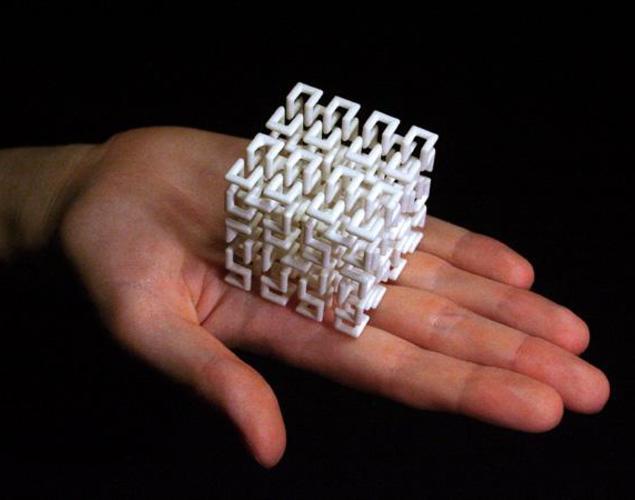
\includegraphics[width=0.75\columnwidth]{images/hilbert3d.jpg}
  \caption{An example of a Hilbert Curve in three dimensions.}
  \label{fig:hilbert3d}
\end{figure}

Space filling curves have direct application in some aspects of image processing and can also be used as patterns for compression or packing.  Used in algorithms for dithering photographs, the Hilbert Curve offers an alternative to scanning and processing the image line by line.  This technique is free of directional features that may be evident in more traditional methods.~\cite[page 103]{Peitgen}.  It also results in aperiodic patterns of clustered dots that are characteristic of
photographic grain.\footnote{Does anyone besides me remember film???}

\section{Design Patterns}  % Target: 3 pages
After a brief introduction to design patterns and their typical use, we will discuss some of the shortcomings of traditional design patterns.  Lastly, we will show how the appropriate use of fractals in design patterns can lead to simpler descriptions of complex systems.

\subsection{Use of Design Patterns}
\subsubsection{History of Design Patterns}
The history of design pattens is most often traced back to Alexander, an architect, who coined the phrase and introduced their use in design and construction of buildings.  
\begin{quote}
  ``Each pattern describes a problem which occurs over and over again in our environment, and then describes the core of the solution to that problem, in such a way that you can use this solution a million times over, without ever doing it the same way twice.''~\cite{Alexander}
\end{quote}

While patterns are most often described in terms of software engineering~\cite{Gamma}, it is clearly the case that they have applicability beyond this traditional domain.  From building architecture to software architecture to systems architecture, pattens simplify our understanding of complex systems in a way that facilitates their decomposition and communication to others.

\subsubsection{Why Use Design Patterns}
There are several things which patterns do for us.  Buschmann, et.\ al., lay out seven characteristics of patterns in the context of software architecture.~\cite{Buschmann}, but they are equally suited to complex systems in general.

\emph{Patterns document proven design experience.}  They don't exist without applicable purpose.  They codify the information that might otherwise exist only among a few experts and allow the novice engineer to apply that knowledge without having to first rediscover it.

\emph{Patterns are abstract.}  Patterns do not map directly onto single components of complex systems. Rather they are representative and descriptive of working ideas within the system.  They are usually not applicable at the component level and may represent several components or subsystems, actions, interactions, and information classes.

\emph{Patterns provide a common vocabulary.}  Especially after a pattern becomes widely adopted, the mere invocation of its name (especially if the name is chosen wisely) conveys a wealth of information quickly, often alleviating the need for one designer to explain the details of a particular solution to another.

\emph{Patterns document architectures.} The vision that you have for the architecture is conveyed in the patterns used to describe it.  ``This helps others to avoid violating this vision when extending or modifying the original architecture\dots''~\cite[page 6]{Buschmann}  The information coded in the pattern is sufficient such that the structure of the solution to the problem is conveyed clearly.

\emph{Patterns support implementation with predefined properties.}  The structure of functional behavior found in patterns helps maintain consistency among cooperating architectural components.  ``In addition, patterns explicitly address nonfunctional requirements for [systems], such as changeability, reliability, testability, or reusability.''~\cite[page 7]{Buschmann}

\emph{Patterns help build complex heterogeneous architectures.}  Think of patterns as building blocks that not only provide physical structure, but also attributes, roles, and relationships.  Using well defined patterns expedites the design and increases the quality of engineered solutions.  

\emph{Patterns help manage complexity.}  By remaining implementation agnostic, patterns provide a plan for how to solve a problem in a way that both breaks down complexity inherent in the problem space and avoids getting mired in implementation details.

So it is no wonder that patterns have such a foothold in the complex world of software engineering.  We can see how these characteristics also benefit the broader, more abstract domain of complex systems engineering.  Establishment and use of appropriate patterns helps us to arrive at and communicate good architectural solutions more quickly by allowing us to leverage the packaged wisdom and experience of tested approaches to recurring problems.

This efficiency affords us do develop more reliable architectures more quickly, with which we can implement solutions to complex problems.  The natural language extension of patterns allows more rapid and accurate communication of complex ideas, independent of implementation details, facilitating the distribution of work across people and organizations.

\subsection{Shortcomings Of Traditional Design Patterns}
The patterns that have been developed mostly to support software architecture are a great place to start and have broad applicability to complex systems engineering and architecture, especially considering that software is often a large component of complex systems.  And like all languages, design patterns are living and organic. So it is natural to extend them in ways that are useful to us.

Despite the wealth of proven design patterns in software architecture, there are plenty of opportunities to improve on and add to the corpus.  Especially given the dynamic nature of the emerging field of complex systems engineering, we are likely to find many new ways to think about and communicate that complexity by applying familiar and relatable patterns.

Since the domain of systems architecture is a proper superset of software architecture, it is likely that the set of design patterns so well suited to the latter would need to be extended to accommodate the former.  In addition, the domain of complex systems likely requires its own design patterns. 

Lastly, traditional patterns tend to address atomic problems in straightforward ways.  While this often makes the patterns easier to read, it creates some unnecessarily complicated architectures.

\begin{quote}
  ``IMHO [sic], the alleged `complexity' (or fragility) of many systems is directly due to the attempt to solve the problem with non-recursive thinking.'' -- Joel Neeley
\end{quote}

Applying recursive thinking through the development of design patterns that are based on fractal structures, we stand to benefit from a significant reduction in complexity.  This reduction in complexity should be on the same order as the reduction characteristic of recursive algorithms like the one presented above.

\subsection{Use of Fractals as Design Patterns}
We have already suggested some of the applicability of fractals to common design problems.  
%TODO: Restate these. (mazzas) Tue Jun 17 11:37:00 2014

What remains is to select some of these that are appropriate and crate full-fledged design patterns around them.

\subsection{Example} % optionally just make a case for further investigation
Work through an example (with figures)

\subsection{From Simplicity, Complexity}
Discuss how simple rules can quickly lead to complexity.

\section{Conclusion}  % Target: 1 page
We have discussed the nature of complexity in engineering and architecture and shown some common methods for dealing with it.  Abstraction and encapsulation provide powerful tools for taming complex systems.  Coding that abstraction and encapsulation into design patterns has been a useful method applied in software architecture for the last two decades and has conspicuous merit in complex systems architecture as well.

Developing recursive design patterns and using fractal structures to represent common and recurring elements of complex architectures offers a way to address the inherent complexity of these problem spaces and extend our vocabulary in meaningful ways that address coordination, communication, and help make success repeatable.

The challenge is to continue to investigate this area and to cultivate a culture of reuse.  There is no reason to derive every solution from first principles when so much experience is available.  Complex problems require complex solutions in order to make them tractable.  Developing recursive, fractal design patterns may significantly reduce this complexity and facilitate communication of complex architectures across domains among practicing engineers.

\bibliography{Mazza_TermPaper}

\end{document}
